\PassOptionsToPackage{dvipsnames,table}{xcolor}
\documentclass[10pt]{beamer}
\usepackage{Cours}

\begin{document}


\input{\detokenize{/home/fenarius/Travail/Cours/cpge-info/latex/MacrosCours.tex}}

% Numéro et titre de chapitre
\setcounter{numchap}{17}
\newcommand{\Ctitle}{\cnum {Graphes}}
\newcommand{\SPATH}{/home/fenarius/Travail/Cours/cpge-info/docs/mp2i/files/C\thenumchap/}
\newcommand{\ar}[1]{\{#1\}}

\makess{Exemples introductifs}
\begin{frame}[fragile]{\Ctitle}{\stitle}
	\begin{block}{Les sept ponts de Konigsberg}
		\begin{center}
			\includegraphics[width=160px]{konigsberg_bridges.eps}\\
			{\footnotesize credit : Wikipedia}
		\end{center}
		Est-il possible de trouver un chemin qui passe une seule fois par chaque pont ?
	\end{block}
\end{frame}

\begin{frame}[fragile]{\Ctitle}{\stitle}
	\begin{block}{Le problème des quatre couleurs}
		\begin{center}
			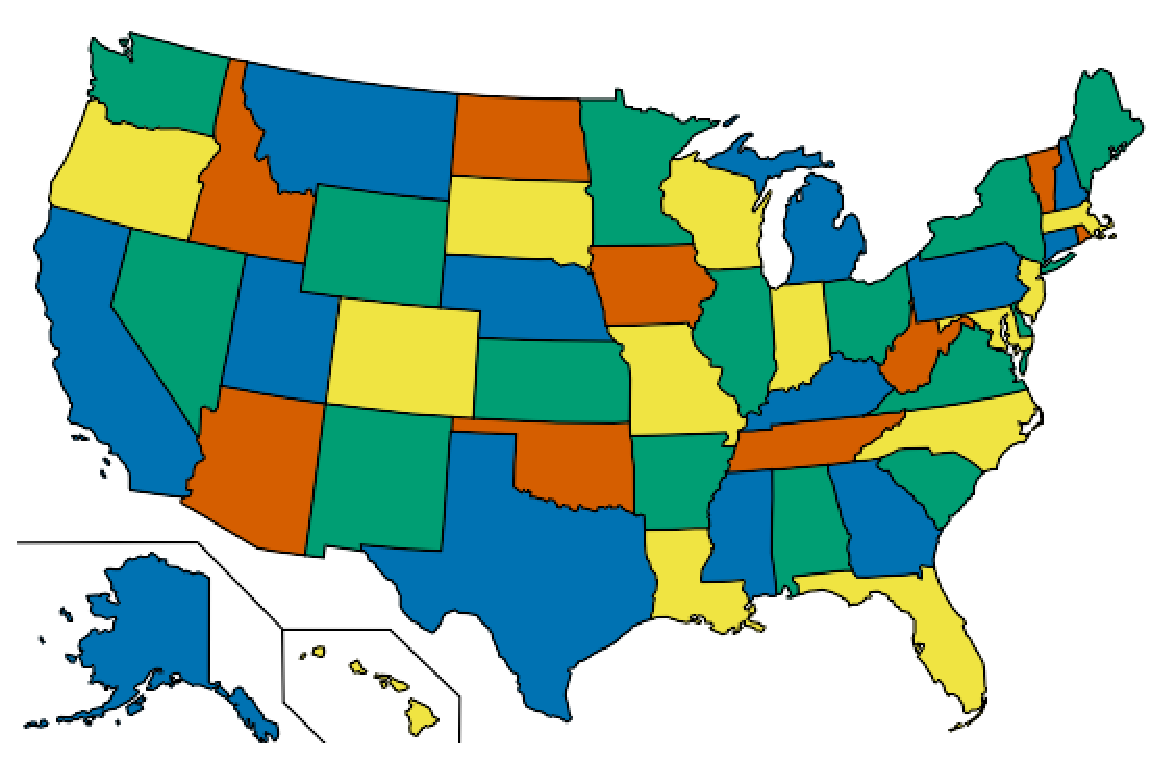
\includegraphics[width=160px]{US4.eps}\\
			{\footnotesize credit : Wikipedia}
		\end{center}
		Peut-on colorier n'importe quelle carte en utilisant seulement 4 couleurs ? (sans que deux pays limitrophes aient la même couleur) 
	\end{block}
\end{frame}

\begin{frame}[fragile]{\Ctitle}{\stitle}
	\begin{block}{Le problème du voyageur de commerce}
		\begin{center}
			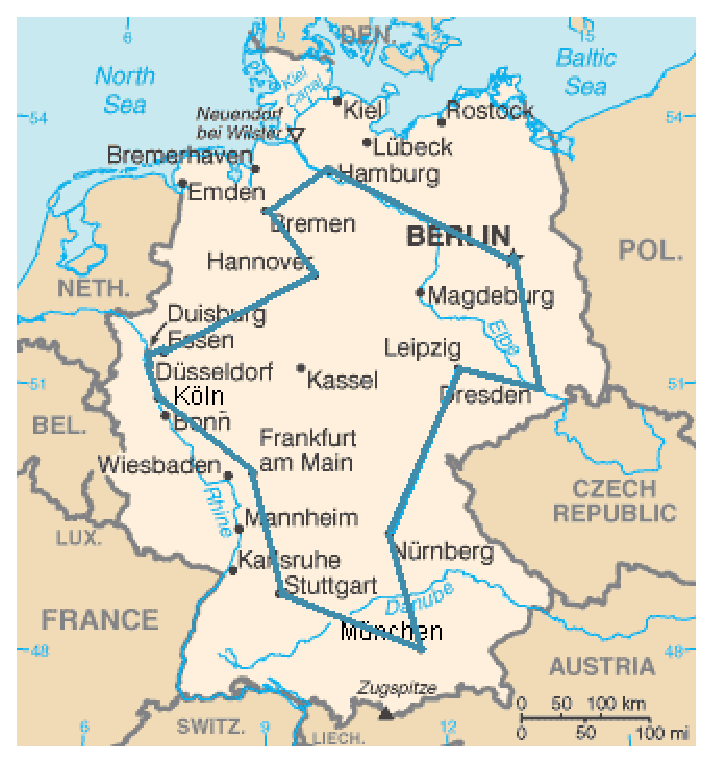
\includegraphics[height=130px]{TSP_Deutschland.eps}\\
			{\footnotesize credit : Wikipedia}
		\end{center}
		Trouver le chemin le plus court possible qui passe par toutes les villes une seule fois et revient à son point de départ.
	\end{block}
\end{frame}


\begin{frame}[fragile]{\Ctitle}{\stitle}
	\begin{block}{Le jeu de Juniper Green}
		\begin{center}
			\includegraphics[width=200px]{juniper5.eps}\\
		\end{center}
		Existe-il une stratégie gagnante au jeu de Juniper Green ?
	\end{block}
\end{frame}

\begin{frame}[fragile]{\Ctitle}{\stitle}
	\begin{block}{Théorie des graphes}
		Ces problèmes se modélisent et se résolvent à l'aide de la \textcolor{blue}{théorie des graphes}, un domaine central de l'informatique ayant des applications variées :
		\begin{itemize}
			\item<1-> {\sc gps} : recherches de chemins,
			\item<2-> planification de tâches,
			\item<3-> réseaux : informatique, sociaux, 
			\item<4-> énergie, transport, \dots
		\end{itemize}
		\onslide<5->{La taille des graphes en jeu impose la recherche d'algorithmes efficaces :}
		\onslide<6->{
		\begin{center}
		\begin{tabularx}{0.7\linewidth}{XXX}
			\textcolor{blue}{Graphe}  & \textcolor{blue}{Sommets} & \textcolor{blue}{Arcs} \\
			\hline 
			\leavevmode{\onslide<7->{Facebook}} & \leavevmode{\onslide<7->{$\simeq 7,2\times 10^8$}} & \leavevmode{\onslide<7->{$\simeq 7\times10^9$}} \\
			\leavevmode{\onslide<8->{OpenStreetMap}} & \leavevmode{\onslide<8->{$\simeq 9\times 10^9$}} & \leavevmode{\onslide<8->{$\simeq 10^9$}} \\
			\leavevmode{\onslide<9->{Jeu d'échecs}} & \leavevmode{\onslide<9->{$\simeq  10^{47}$}} & \leavevmode{\onslide<9->{?}} \\
		\end{tabularx}
	\end{center}}
	\end{block}
\end{frame}

\makess{Définition et vocabulaire des graphes}
\begin{frame}[fragile]{\Ctitle}{\stitle}
\begin{alertblock}{Définition}
    \onslide<1->{Un \textcolor{red}{graphe non-orienté} est la donnée :}
    \begin{itemize}
        \item<2->{D'un ensemble de \textcolor{blue}{sommets} (ou \textcolor{blue}{n\oe{}uds}) $S$ fini (\textcolor{gray}{V pour \textit{vertice} en anglais.}).}
        \item<3->{D'un ensemble de paires de sommets $A$ appelés \textcolor{blue}{arêtes} (\textcolor{gray}{E pour \textit{edges} en anglais}).}
    \end{itemize}
\end{alertblock}
	\onslide<4->{\begin{block}{Remarques}
		\begin{itemize}
			\item<5-> Une arête est donc une paire $\{x, y \}$, avec $x \in S$, $y \in S$ et $x \neq y$. 
			\item<6-> Puisque $\{x, y \} = \{ y, x \}$, l'ordre n'a pas d'importance.
			\item<7-> On notera $ x \relbar y$ ou plus simplement $xy$ l'arête $\{x, y \}$.
		\end{itemize}
	\end{block}}
\end{frame}

% Premiers exemples
\begin{frame}[fragile]{\Ctitle}{\stitle}
\begin{exampleblock}{Exemple}
    \begin{pspicture}(0,2)(5,4)
        \rput(0.2,2.8){\Circlenode{S1}{$a$}}
        \rput(2,3){\Circlenode{S2}{$b$}}
        \rput(4,2){\Circlenode{S3}{$c$}} 
        \rput(8,3){\Circlenode{S4}{$d$}}
        \rput(7,2){\Circlenode{S5}{$e$}}
        \rput(6,3){\Circlenode{S6}{$f$}}
        \rput(4,3.5){\circlenode{S7}{$g$}}
        \ncarc{-}{S4}{S5}
        \ncarc{-}{S6}{S4} 
        \ncarc{-}{S1}{S2}
        \ncarc{-}{S2}{S3}
        \ncarc{-}{S2}{S7}
		\ncarc{-}{S7}{S3}
    \end{pspicture}\\
    \onslide<2->{$S = \{a,b,c,d,e,f,g\}$ \\}
    \onslide<3->{$A = \{\ar{a,b},\ar{b,c},\ar{b,g},\ar{c,g},\ar{f,d},\ar{e,d}\}$\bigskip \\}
	\onslide<4->{Dessiner le graphe $G'$ définit par $S' = \{1, 2, 3, 4\}$ et $A' = \{\ar{1,2},\ar{3,4},\ar{1,4}\}$}
	\onslide<5->{
		\begin{pspicture}(0,0)(2,2)
			\rput(1,0.5){\Circlenode[linecolor=OliveGreen]{T1}{$\textcolor{OliveGreen}{1}$}}
			\rput(1,1.5){\Circlenode[linecolor=OliveGreen]{T2}{$\textcolor{OliveGreen}{2}$}}
			\rput(4,0.5){\Circlenode[linecolor=OliveGreen]{T3}{$\textcolor{OliveGreen}{3}$}}
			\rput(4,1.5){\Circlenode[linecolor=OliveGreen]{T4}{$\textcolor{OliveGreen}{4}$}}
		\end{pspicture}\\
		\ncline[linecolor=OliveGreen]{-}{T1}{T2}
		\ncline[linecolor=OliveGreen]{-}{T3}{T4}
		\ncline[linecolor=OliveGreen]{-}{T1}{T4}
	}
    \onslide<6->{\textcolor{BrickRed}{\small \danger} L'emplacement des n\oe{}uds sur la représentation graphique n'a pas d'importance.}
\end{exampleblock}
\end{frame}


\begin{frame}[fragile]{\Ctitle}{\stitle}
	\begin{block}{Vocabulaire}
		\begin{itemize}
			\item<1-> L'\textcolor{blue}{ordre} d'un graphe est son nombre de sommets.
			\item<2-> Les \textcolor{blue}{voisins} d'un sommet $s$ est l'ensemble ${\cal V}(s) = \{t \in S  \text{ tel que } s \relbar t\}$.
			\item<3-> Le \textcolor{blue}{degré} d'un sommet $s$ noté $d(s)$ est son nombre de voisins $d(s) = |{\cal V}(s)|$.
		\end{itemize}
	\end{block}
	\onslide<4->{
	\begin{exampleblock}{Exercices}
		\begin{enumerate}
			\item<4-> Dessiner un graphe d'ordre 5 dont tous les sommets sont de degrés 2.
			\item<5-> Donner un majorant du nombre d'arêtes d'un graphe d'ordre $n$.  
		\end{enumerate}}
	\end{exampleblock}
\end{frame}

% Implémentation des graphes par matrice d'adjacence
\makess{Représentations en machine}
\begin{frame}[fragile]{\Ctitle}{\stitle}
	\begin{alertblock}{Représentation par matrice d'adjacence}
		Soit un graphe $G=(S,A)$ avec $|S|=n$, on note $S = \{x_0,\dots,x_{n-1}\}$.  La \textcolor{blue}{matrice d'adjacence} du graphe $G$ est la matrice carrée d'ordre $n$, $M$  définie par : $M_{ij} = 1$ si $\ar{x_i,x_j} \in A$ et $M_{ij} = 0$ sinon. \\
		\onslide<2->$M$ est une matrice symétrique.
	\end{alertblock}
	\onslide<3->{
	\begin{exampleblock}{Exemple : Un graphe et sa matrice d'adjacence}
			\begin{pspicture}(-2,0)(5,2)
				\rput(1,0.5){\Circlenode{S1}{$x_1$}}
				\rput(1,1.5){\Circlenode{S2}{$x_2$}}
				\rput(4,0.5){\Circlenode{S3}{$x_3$}}
				\rput(4,1.5){\Circlenode{S4}{$x_4$}}
				\rput(2.5,1){\Circlenode{S0}{$x_0$}}
				\ncline{-}{S0}{S1}
				\ncline{-}{S0}{S2}
				\ncline[linecolor=red]{-}{S0}{S3}
				\ncline{-}{S1}{S3}
				\ncline{-}{S2}{S4}
				\rput(7,1){$\begin{pmatrix}
					0 & 1 & 1 & \textcolor{red}{1} & 0 \\
					1 & 0 & 0 & 1 & 0 \\
					1 & 0 & 0 & 0 & 1 \\
					\textcolor{red}{1} & 1 & 0 & 0 & 0 \\
					0 & 0 & 1 & 0 & 0 \\
				\end{pmatrix}$}
			\end{pspicture} 
	\end{exampleblock}}
\end{frame}

\begin{frame}[fragile]{\Ctitle}{\stitle}
	\begin{exampleblock}{Exemple}
		\begin{enumerate}
			\item<1-> En supposant les sommets numérotés dans l'ordre alphabétique, écrire la matrice d'adjacence du graphe suivant :
				\begin{center}
					\begin{pspicture}(5,2)
						\rput(0,1.8){\circlenode{A}{A}}
						\rput(1,0.5){\circlenode{E}{E}}
						\rput(2,1){\circlenode{B}{B}}
						\rput(4,0.7){\circlenode{D}{D}}
						\rput(6,1.5){\circlenode{C}{C}}
						\ncarc{-}{A}{E}
						\ncarc{-}{A}{B}
						\ncarc{-}{A}{C}
						\ncarc[arcangle=-10]{-}{B}{D}
						\ncarc{-}{C}{B}
						\ncarc[arcangle=-10]{-}{D}{C}
						\ncarc[arcangleA=-45,arcangleB=-40]{-}{E}{C}
						\ncline{-}{E}{B}
					\end{pspicture}
				\end{center}
			\item<2-> Dessiner le graphe ayant la matrice d'adjacence suivante (on appellera les sommets $x_0, x_1, \dots $) :\\
				$\begin{pmatrix}
						0 & 0 & 1 & 1 & 1 \\
						1 & 0 & 1 & 0 & 0 \\
						1 & 1 & 0 & 0 & 1 \\
						1 & 0 & 0 & 1 & 0 \\
						0 & 0 & 1 & 0 & 0 \\
					\end{pmatrix}$
		\end{enumerate}
	\end{exampleblock}
\end{frame}

\begin{frame}[fragile]{\Ctitle}{\stitle}
	\begin{block}{Implémentation en C : tableau statique}
		\onslide<2->{\inputpartC{\SPATH/madj_stat.c}{}{\small}{5}{6}}
		\onslide<3->{On évite ainsi l'utilisation de pointeurs et on manipule directement la matrice d'adjacence. On doit passer la taille effective du graphe aux fonctions lorsque nécessaire.}
	\end{block}
	\onslide<4->{
	\begin{exampleblock}{Exemple}
		Ecrire la fonction de signature \mintinline{c}{void cree_arete(graphe g, int i, int j)} qui crée l'arête reliant les sommets {\tt i} et {\tt j}.
		\onslide<5->{\inputpartC{\SPATH/madj_stat.c}{}{\small}{19}{21}}
	\end{exampleblock}}
\end{frame}

\begin{frame}[fragile]{\Ctitle}{\stitle}
	\begin{block}{Implémentation en C : type structuré}
	On utilise un \mintinline{c}{struct} contenant un champ \mintinline{c}{int} (le nombre de sommets), et un pointeur vers la matrice d'adjacence linéarisée.
	\onslide<2->{L'indice de $M_{ij}$ dans la matrice linéarisée est alors $i\times |S| +j$.}
	\onslide<3->{\inputpartC{\SPATH/madj_dyn.c}{}{\small}{5}{10}}
	\onslide<4->{Cette solution est plus efficace en terme de d'utilisation mémoire mais impose l'utilisation de pointeurs.}
	\end{block}
\end{frame}

\begin{frame}{\Ctitle}{\stitle}
	\begin{exampleblock}{Exemple}
		Pour initialiser une variable de type graphe lorsque le nombre de sommets est connu, on propose la solution suivante :
		\onslide<2->{\inputpartC{\SPATH/madj_dyn.c}{}{\small}{12}{18}}
		\onslide<3->{Ecrire la fonction {\tt detruit\_graphe} qui permet de libérer la mémoire allouée par la fonction d'initialisation ci-dessus}
		\onslide<4->{\inputpartC{\SPATH/madj_dyn.c}{}{\small}{20}{21}}
	\end{exampleblock}
\end{frame}

% Exemple de matrice d'adjacences
\begin{frame}[fragile]{\Ctitle}{\stitle}
	\begin{block}{Implémentation en OCaml}
		\begin{itemize}
			\item<1->On crée le type graphe sous forme d'un type structuré
			\onslide<2->{\inputpartOCaml{\SPATH/madj.ml}{}{\small}{1}{3}}
			\item<3->La création d'un graphe peut alors se faire à l'aide d'une fonction d'initialisation
			\onslide<4->{\inputpartOCaml{\SPATH/madj.ml}{}{\small}{5}{6}}
			\onslide<5->{\textcolor{BrickRed}{\small \danger \;}{On rappelle qu'on initialise avec \mintinline{ocaml}{Array.make_matrix} afin d'éviter le problème des références multiples à une même ligne.} }
		\end{itemize}
	\end{block}
\end{frame}

\begin{frame}[fragile]{\Ctitle}{\stitle}
	\begin{exampleblock}{Exemples}
		\begin{enumerate}
			\item<1-> Ecrire la fonction {\tt cree\_arete : graphe -> int -> int -> unit} qui crée une arête dans un graphe.
			\onslide<2->{\inputpartOCaml{\SPATH/madj.ml}{}{\small}{23}{25}}
			\item<1-> Ecrire une fonction {\tt degre : graphe -> int -> int} qui renvoie le degré d'un sommet.
			 \onslide<2->{\inputpartOCaml{\SPATH/madj.ml}{}{\small}{27}{32}}
		\end{enumerate}
	\end{exampleblock}
\end{frame}

% Implémentation des graphes par liste d'adjacence
\begin{frame}[fragile]{\Ctitle}{\stitle}
	\begin{alertblock}{Représentation par listes d'adjacence}
		On peut représenter un graphe à l'aide de listes d'adjacences, c'est à dire en mémorisant pour chaque sommet du graphe la liste de ses voisins.\\
		\onslide<2->{Un graphe $G=(S,A)$ est alors un tableau de taille $|S|$ où la case d'indice $i$ contient la liste des voisins du sommet $x_i$.}
	\end{alertblock}
	\onslide<4->{
	\begin{exampleblock}{Exemple : Un graphe et ses listes d'adjacence}
		\begin{pspicture}(-2,0)(5,2)
			\rput(1,0.5){\Circlenode{S1}{$x_1$}}
			\rput(1,1.5){\Circlenode{S2}{$x_2$}}
			\rput(4,0.5){\Circlenode{S3}{$x_3$}}
			\rput(4,1.5){\Circlenode{S4}{$x_4$}}
			\rput(2.5,1){\Circlenode{S0}{$x_0$}}
			\ncline{-}{S0}{S1}
			\ncline[linecolor=red]{-}{S0}{S2}
			\ncline{-}{S0}{S3}
			\ncline{-}{S1}{S3}
			\ncline{-}{S2}{S4}
			\rput(7,1){\begin{tabular}{lcl}
				0 &$\rightarrow$ & {\tt [1; \textcolor{red}{2}; 3]} \\
				1 &$\rightarrow$ & {\tt [0; 3]} \\
				2 &$\rightarrow$ &{\tt [\textcolor{red}{0}; 4]} \\
				3 &$\rightarrow$ &{\tt [0; 1]} \\
				4 &$\rightarrow$ &{\tt [2]} \\
			\end{tabular}}
		\end{pspicture} 
\end{exampleblock}}
\end{frame}

% Exemple de liste d'adjacences
\begin{frame}[fragile]{\Ctitle}{\stitle}
	\begin{exampleblock}{Exemple}
		\begin{enumerate}
			\item<1-> Ecrire les listes d'adjacences du graphe suivante :
			\begin{center}
				\begin{pspicture}(5,2)
					\rput(0,1.8){\circlenode{A}{A}}
					\rput(1,0.5){\circlenode{E}{E}}
					\rput(2,1){\circlenode{B}{B}}
					\rput(4,0.7){\circlenode{D}{D}}
					\rput(6,1.5){\circlenode{C}{C}}
					\ncarc{-}{A}{E}
					\ncarc{-}{A}{B}
					\ncarc{-}{A}{C}
					\ncarc[arcangle=-10]{-}{B}{D}
					\ncarc{-}{C}{B}
					\ncarc[arcangle=-10]{-}{D}{C}
					\ncarc[arcangleA=-45,arcangleB=-40]{-}{E}{C}
					\ncline{-}{E}{B}
				\end{pspicture}
			\end{center}
			\item<2-> Dessiner le graphe représenté par le tableau $T$ tel que :	\\			
{\tt 
	T[0] = [2] \\
 	T[1] = [3; 4] \\
 	T[2] = [0; 1] \\
 	T[3] = [1; 2] \\
 	T[4] = [1; 2]\\
} 
		\end{enumerate}
	\end{exampleblock}
\end{frame}

\begin{frame}[fragile]{\Ctitle}{\stitle}
	\begin{block}{Implémentation en C : tableau statique d'entiers}
		\onslide<2->{\inputpartC{\SPATH/ladj_stat.c}{}{\small}{5}{8}}	
		\onslide<3->{On évite de cette façon l'utilisation de pointeurs mais au prix d'un manque d'efficacité en terme d'occupation mémoire.}
	\end{block}
	\onslide<4->{\begin{exampleblock}{Exemple : Un graphe et sa matrice d'adjacence}
		\begin{pspicture}(-2,0)(5,2)
			\rput(1,0.5){\Circlenode{S1}{$x_1$}}
			\rput(1,1.5){\Circlenode{S2}{$x_2$}}
			\rput(4,0.5){\Circlenode{S3}{$x_3$}}
			\rput(4,1.5){\Circlenode{S4}{$x_4$}}
			\rput(2.5,1){\Circlenode{S0}{$x_0$}} \nput[labelsep=1 pt]{-25}{S0}{\textcolor{blue}{\footnotesize $2$}}
			\ncline[linecolor=red]{-}{S0}{S4}
			\ncline[linecolor=red]{-}{S0}{S2}
			\ncline{-}{S1}{S2}
			\ncline{-}{S1}{S3}
			\ncline{-}{S2}{S4}
			\ncline{-}{S3}{S4}
			\rput(7,1){$\begin{pmatrix}
				\textcolor{blue}{2} & \textcolor{red}{2} & \textcolor{red}{4} & \textcolor{gray}{0} & \textcolor{gray}{0} \\
				2 & 2 & 3 & \textcolor{gray}{0} & \textcolor{gray}{0} \\
				3 & 0 & 1 & 4 & \textcolor{gray}{0} \\
				\alt<5->{2}{?} & \alt<5->{1}{?} & \alt<5->{4}{?} & \alt<5->{\textcolor{gray}{0}}{?} & \alt<5->{\textcolor{gray}{0}}{?} \\
				\alt<5->{3}{?} & \alt<5->{2}{?} & \alt<5->{0}{?} & \alt<5->{3}{?} & \alt<5->{\textcolor{gray}{0}}{?} \\
			\end{pmatrix}$}
		\end{pspicture} 
\end{exampleblock}}
\end{frame}

\begin{frame}[fragile]{\Ctitle}{\stitle}
	\begin{exampleblock}{Exemples}
		\begin{enumerate}
		\item<1->Ecrire la fonction de signature \mintinline{c}{int degre(graphe g, int i)} qui renvoie le degré du sommet de numéro {\tt i}.
		\onslide<2->{\inputpartC{\SPATH/ladj_stat.c}{}{\small}{66}{69}}	
		\item<1->Ecrire la fonction de signature \mintinline{c}{void cree_arete(graphe g, int i, int j)} qui crée l'arête entre les sommets {\tt i} et {\tt j} dans le graphe {\tt g}
		\onslide<3->{\inputpartC{\SPATH/ladj_stat.c}{}{\small}{17}{21}}	
		\end{enumerate}
	\end{exampleblock}
\end{frame}

\begin{frame}[fragile]{\Ctitle}{\stitle}
	\begin{block}{Implémentation en C : tableau de listes chainées}
		On utilise un tableau de liste chainées afin d'optimiser l'espace mémoire occupé :
		\onslide<2->{\inputpartC{\SPATH/ladj_dyn.c}{}{\small}{10}{13}}
		\onslide<3->{\textcolor{blue}{\small \rappel\;}{ On rappelle la structure de liste chainée : }}
		\onslide<3->{\inputpartC{\SPATH/ladj_dyn.c}{}{\small}{4}{8}}
	\end{block}
\end{frame}

\begin{frame}[fragile]{\Ctitle}{\stitle}
	\begin{block}{Implémentation en OCaml}
		On utilise le type \mintinline{ocaml}{list} de OCaml
		\onslide<2->{\inputpartOCaml{\SPATH/ladj.ml}{}{\small}{1}{3}}
		\onslide<3->{On peut alors écrire une fonction de création d'un graphe de taille {\tt n} :}
		\onslide<4->{\inputpartOCaml{\SPATH/ladj.ml}{}{\small}{6}{7}}
	\end{block}
	\onslide<5->{
	\begin{exampleblock}{Exemple}
		Ecrire la fonction {\tt cree\_arete : graphe -> int -> int -> unit}
		\onslide<6->{\inputpartOCaml{\SPATH/ladj.ml}{}{\small}{9}{11}}
	\end{exampleblock}}
\end{frame}

\begin{frame}[fragile]{\Ctitle}{\stitle}
	\begin{block}{Comparatif}
		\begin{tabular}{|l|c|c|}
			\cline{2-3}
			\multicolumn{1}{c|}{} & Matrice d'adjacence & Liste d'adjacence \\
			\hline
			Occupation mémoire  & $O(|S|^2)$ & $O(|S|+|A|)$ \\
			Modification d'arête & $O(1)$ & $O(|S|)$ \\
			Test d'existence d'une arête & $O(1)$ & $O(|S|)$ \\
			Enumération des voisins & $O(|S|)$ & $O(1)$ \\
			\hline
		\end{tabular}\\
		\onslide<2->Un choix d'implémentation doit donc tenir compte :
		\begin{itemize}
			\item<3-> de l'ordre du graphe 
			\item<4-> de la \textit{\og{} densité\fg{}} du graphe
			\item<5-> des algorithmes utilisés
		\end{itemize}
		\onslide<6->{\textcolor{red}{\small \danger \;} Les complexités spatiales et temporelles des algorithmes dépendent de la représentation choisie !} \\
		\onslide<7->{Par exemple, le test d'existence d'une arête est une opération élémentaire dans  le cas représentation par matrice d'adjacence et est de complexité linéaire (en $|S|$), dans le cas des listes d'adjacences.}
	\end{block}
\end{frame}

\makess{Graphes orientés}
\begin{frame}[fragile]{\Ctitle}{\stitle}
	\begin{block}{Relation non symétrique}
		Dans de nombreuses situations (voie à sens unique, lien d'un site web à un autre, relation \textit{\og{} follower \fg{}} dans un réseau social, \dots), on doit modéliser sur un ensemble $S$, des relations non symétriques, ce qui conduit à la notion de graphe orienté.
	\end{block}
	\onslide<2->{
	\begin{alertblock}{Définition}
		\onslide<2->{Un \textcolor{red}{graphe orienté} est la donnée :}
    \begin{itemize}
        \item<3->{D'un ensemble de \textcolor{blue}{sommets} (ou \textcolor{blue}{n\oe{}uds}) $S$ fini.}
        \item<4->{D'un ensemble de \textbf{couples} de sommets $A \subset S\times S$ appelés \textcolor{blue}{arcs}}
    \end{itemize}
	\onslide<5-> L'ordre est important, $(x,y) \neq (y,x)$, on notera un arc $x \rightarrow y$ ou $xy$.
	\end{alertblock}}
\end{frame}

\begin{frame}[fragile]{\Ctitle}{\stitle}
	\begin{exampleblock}{Exemple}
		\vspace{0.2cm}
		\begin{pspicture}(-2,-2)(2,2)
			\rput(0,2){\Circlenode{T1}{$a$}}
			\rput(-1.5,0.9){\Circlenode{T2}{$b$}}
			\rput(1,-1){\Circlenode{T4}{$d$}}
			\rput(-1,-1){\Circlenode{T3}{$c$}}
			\rput(1.5,0.9){\Circlenode{T5}{$e$}}
		\end{pspicture}
		\ncline{->}{T1}{T2}
		\ncline{->}{T2}{T3}
		\ncline{->}{T3}{T4}
		\ncline{->}{T4}{T5}
		\ncline{->}{T5}{T1}
		\ncarc{->}{T1}{T3}
		\ncarc{->}{T1}{T4}
		\ncarc{->}{T4}{T1} \vspace{-0.7cm}
		\begin{itemize}
			\item $S = \{a, b, c, d ,e\}$
			\item $A = \{ (a,b), (b,c), (c,d), (d,e), (e,a), (a,c), (a,d), (d,a)\}$
		\end{itemize}
	\end{exampleblock}
	
\end{frame}


\begin{frame}[fragile]{\Ctitle}{\stitle}
	\begin{block}{Vocabulaire}
		\begin{itemize}
			\item<2-> Les \textcolor{blue}{successeurs} (ou \textcolor{blue}{voisins sortants}) d'un sommet $s \in S$ sont les éléments de l'ensemble ${\cal V_{+}}(s) = \{t \in S  \text{ tel que } s \to t\}$.
			\item<3-> Le \textcolor{blue}{degré sortant} d'un sommet $s$ noté $d_+(s)$ est son nombre de sucesseurs $d_+(s) = |{\cal V_+}(s)|$.
			\item<4-> Les \textcolor{blue}{prédecesseurs} (ou \textcolor{blue}{voisins entrants}) d'un sommet $s \in S$ sont les éléments de l'ensemble ${\cal V_{-}}(s) = \{t \in S  \text{ tel que } t \to s\}$.
			\item<5-> Le \textcolor{blue}{degré entrant} d'un sommet $s$ noté $d_-(s)$ est son nombre de prédecesseurs $d_-(s) = |{\cal V_-}(s)|$.
			\item<6-> Les \textcolor{blue}{voisins} d'un sommet $s$ sont les éléments de ${\cal V}(s) = {\cal V_+}(s) \cup {\cal V_-}(s) $
			\item<7-> Le \textcolor{blue}{degré} d'un sommet $s$ noté $d(s)$ est la somme de ses degrés entrants et sortants $d(s) = d_-(s)+d_+(s)$
		\end{itemize}
	\end{block}
\end{frame}

\begin{frame}[fragile]{\Ctitle}{\stitle}
	\begin{exampleblock}{Exemple}
		\vspace{0.2cm}
		\begin{pspicture}(-2,-2)(2,2)
			\rput(0,2){\Circlenode{T1}{$a$}}
			\rput(-1.5,0.9){\Circlenode{T2}{$b$}}
			\rput(1,-1){\Circlenode{T4}{$d$}}
			\rput(-1,-1){\Circlenode{T3}{$c$}}
			\rput(1.5,0.9){\Circlenode{T5}{$e$}}
		\end{pspicture}
		\ncline{->}{T1}{T2}
		\ncline{->}{T2}{T3}
		\ncline{->}{T3}{T4}
		\ncline{->}{T4}{T5}
		\ncline{->}{T5}{T1}
		\ncarc{->}{T1}{T3}
		\ncarc{->}{T1}{T4}
		\ncarc{->}{T4}{T1} \vspace{-0.7cm}
		\begin{itemize}
			\item<2-> $V_+(a)= $ \alt<6->{\textcolor{OliveGreen}{$\{b,c,d\}$}}{?}
			\item<3-> $V_+(d)= $ \alt<7->{\textcolor{OliveGreen}{$\{a,c\}$}}{?}
			\item<4-> $d_+(e)= $  \alt<8->{\textcolor{OliveGreen}{$1$}}{?}
			\item<5-> $d_-(a)= $  \alt<9->{\textcolor{OliveGreen}{$2$}}{?}
		\end{itemize}
	\end{exampleblock}
\end{frame}

\begin{frame}[fragile]{\Ctitle}{\stitle}
	\begin{block}{Représentation informatique}
		\begin{itemize}
			\item La représentation par matrice d'adjacence reste valide mais la matrice n'est plus nécessairement symétrique.
			\item<2-> Dans la représentation par liste d'adjacence, les listes contiennent les \textcolor{BrickRed}{voisins sortants}.
			\item<3-> Les remarques sur le choix d'une représentation restent valides.\\
			\onslide<4->{\textcolor{red}{\small \danger} Attention cependant, dans le cas des listes d'adjacence on a un accès en $O(1)$ à la liste des voisins \textbf{sortants}, lister les voisins entrants s'avère plus compliqué (voir TP).}
		\end{itemize}
	\end{block}
\end{frame}


\makess{Graphes pondérés}
\begin{frame}[fragile]{\Ctitle}{\stitle}
	\begin{block}{Graphes pondérés}
		Dans de nombreuses situations (distance entre deux villes, capacité d'une liaison dans un réseau, \dots), on souhaite pouvoir ajouter des informations aux  arêtes d'un graphe, ce qui conduit à la notion de graphe pondéré (orienté ou non).
	\end{block}
	\onslide<2->
	{\begin{alertblock}{Définition}
		Etant donné un graphe $G=(S,A)$n une fonction de pondération de $G$ est un fonction $\omega : A \mapsto \R$. Le \textcolor{blue}{poids} de l'arête (ou arc) $a$ est le réel $w(a)$ et on dit que $(G,S,\omega)$ est un \textcolor{blue}{graphe pondéré}
	\end{alertblock}}
\end{frame}

\begin{frame}[fragile]{\Ctitle}{\stitle}
	\begin{exampleblock}{Exemple}
		\begin{pspicture}(0,-2.2)(5,2.2)
		\rput(1,2){\circlenode{R1}{$S_1$}}
		\rput(3,2){\circlenode{R2}{$S_2$}}
		\rput(1,0){\circlenode{R3}{$S_3$}}
		\rput(3,0){\circlenode{R4}{$S_4$}}
		\rput(5,0){\circlenode{R5}{$S_5$}}
		\rput(1,-2){\circlenode{R6}{$S_6$}}
		\rput(3,-2){\circlenode{R7}{$S_7$}}
		\rput(5,-2){\circlenode{R8}{$S_8$}}
		\ncline{R1}{R2} \naput[labelsep=0.06]{\textcolor{blue}{2}}
		\ncline{R1}{R3} \naput[labelsep=0.06]{\textcolor{blue}{1}}
		\ncline{R1}{R4} \naput[labelsep=0.06]{\textcolor{blue}{3}}
		\ncline{R2}{R4} \naput[labelsep=0.06]{\textcolor{blue}{5}}
		\ncline{R3}{R4} \naput[labelsep=0.06]{\textcolor{blue}{1}}
		\ncline{R3}{R6} \naput[labelsep=0.06]{\textcolor{blue}{7}}
		\ncline{R3}{R7} \naput[labelsep=0.06]{\textcolor{blue}{7}}
		\ncline{R4}{R5} \naput[labelsep=0.06]{\textcolor{blue}{2}}
		\ncline{R4}{R7} \naput[labelsep=0.06]{\textcolor{blue}{6}}
		\ncline{R4}{R8} \naput[labelsep=0.06]{\textcolor{blue}{7}}
		\ncline{R5}{R8} \naput[labelsep=0.06]{\textcolor{blue}{4}}
		\ncline{R6}{R7} \naput[labelsep=0.06]{\textcolor{blue}{4}}
		\ncline{R7}{R8} \naput[labelsep=0.06]{\textcolor{blue}{9}}
	\end{pspicture}
	\end{exampleblock}
\end{frame}

\begin{frame}[fragile]{\Ctitle}{\stitle}
	\begin{block}{Représentation informatique}
		En pratique, on se limitera le plus souvent à des poids entiers et positifs.
		\begin{itemize}
			\item<1-> Dans le cas d'une représentation par matrice d'adjacence, on posera :
			$M_{ij} = \left\{
				\begin{array}{ll}
				0 & \text{ si } i =j  \\
				\omega(ij) & \text{ si } i \neq j \text{ et } ij \in A \\
				+\infty & \text{ sinon } \\
				\end{array}
				\right.$ 
			\item<2-> Dans le cas d'une représentation par liste d'adjacence, on stocke dans la liste d'adjacence d'un sommet $s$, les couples $(t, \omega(st))$ 
		\end{itemize}
		\onslide<3->{\textcolor{red}{\small \danger\;}{L'absence d'arc est indiqué par un 0 dans la matrice d'adjacence d'un graphe non pondéré et par un $+\infty$ dans celle d'un graphe pondéré.}}
	\end{block}
\end{frame}

\begin{frame}[fragile]{\Ctitle}{\stitle}
\begin{exampleblock}{Exemple : Un graphe orienté pondéré et sa matrice d'adjacence}
	\begin{pspicture}(-1,0)(5,2)
		\rput(1,0.2){\Circlenode{S1}{$S_1$}}
		\rput(1,1.8){\Circlenode{S2}{$S_2$}}
		\rput(4,0.2){\Circlenode{S3}{$S_3$}}
		\rput(4,1.8){\Circlenode{S4}{$S_4$}}
		\rput(2.5,1){\Circlenode{S0}{$S_0$}}
		\ncline{->}{S1}{S3} \naput[labelsep=0.07]{{\footnotesize 7}}
		\ncline{->}{S2}{S0} \naput[labelsep=0.07]{{\footnotesize 5}}
		\ncline{->}{S0}{S3} \naput[labelsep=0.07]{{\footnotesize 8}}
		\ncline{->}{S0}{S4} \naput[labelsep=0.07]{{\footnotesize 2}}
		\ncline{->}{S4}{S2} \nbput[labelsep=0.07]{{\footnotesize 1}}
		\ncline{->}{S1}{S2} \naput[labelsep=0.07]{\textcolor{blue}{\footnotesize 2}}
		\rput(8,1){$\begin{pmatrix}
			0 & +\infty & +\infty & 8 & 2 \\
			+\infty & 0 & \textcolor{blue}{2} & 7 & +\infty \\
			5 & +\infty & 0 & +\infty & +\infty \\
			+\infty & +\infty & +\infty & 0 & +\infty \\
			+\infty & +\infty & 1 & +\infty & 0 \\
		\end{pmatrix}$}
	\end{pspicture} 
\end{exampleblock}
\end{frame}

\makess{Parcours de graphes}
\begin{frame}[fragile]{\Ctitle}{\stitle}
	\begin{block}{Parcours d'un graphe}
		A la base des algorithmes sur les graphes, on trouve les parcours de graphe, c'est à dire l'exploration des sommets. A partir du sommet de départ, on peut :
		\begin{itemize}
			\item<1-> explorer tous ses voisins immédiats, puis les voisins des voisins et ainsi de suite. Le graphe est donc exploré en \og cercle concentrique\fg autour du sommet de départ  \dots, on parle alors de  \textcolor{blue}{parcours en largeur} ou \textcolor{gray}{breadth first search (\textit{BFS})} en anglais.
			\item<2-> explorer à chaque étape le premier voisin non encore exploré. Lorsque qu'on atteint un sommet dont tous les voisins ont déjà été exploré, on revient en arrière, on parle alors de  \textcolor{blue}{parcours en profondeur} ou \textcolor{gray}{depth first search (\textit{DFS})} en anglais.
		\end{itemize}
	\end{block}
\end{frame}


% Vocabulaire

	
	

\begin{frame}[fragile]{\Ctitle}{\stitle}
		\begin{exampleblock}{Exemple de parcours en largeur}
			\begin{center}
					\begin{pspicture}(5,2)
						\rput(0,1.8){\circlenode[linewidth=1pt,linecolor=red,fillcolor=fluo,fillstyle=solid]{A}{A}}
						\rput(1,0.5){\circlenode{E}{E}}
						\rput(2,1){\circlenode{B}{B}}
						\rput(4,0.7){\circlenode{D}{D}}
						\rput(6,1.5){\circlenode{C}{C}}
						\ncarc{->}{A}{E}
						\ncarc{->}{A}{B}
						\ncarc{->}{A}{C}
						\ncarc[arcangle=-10]{->}{B}{D}
						\ncarc{->}{C}{B}
						\ncarc[arcangle=-10]{->}{D}{C}
						\ncarc[arcangleA=-45,arcangleB=-40]{->}{E}{C}
						\ncline{->}{E}{B}
					\end{pspicture}
				\end{center}
		Sommets explorés : \fbox{A}
		\end{exampleblock}
\end{frame}

\begin{frame}[fragile]{\Ctitle}{\stitle}
	\begin{exampleblock}{Exemple de parcours en largeur}
		\begin{center}
				\begin{pspicture}(5,2)
					\rput(0,1.8){\circlenode[linewidth=1pt,linecolor=red,fillcolor=fluo,fillstyle=solid]{A}{A}}
					\rput(1,0.5){\circlenode[linewidth=1pt,linecolor=red,fillcolor=fluo,fillstyle=solid]{E}{E}}
					\rput(2,1){\circlenode[linewidth=1pt,linecolor=red,fillcolor=fluo,fillstyle=solid]{B}{B}}
					\rput(4,0.7){\circlenode{D}{D}}
					\rput(6,1.5){\circlenode[linewidth=1pt,linecolor=red,fillcolor=fluo,fillstyle=solid]{C}{C}}
					\ncarc{->}{A}{E}
					\ncarc{->}{A}{B}
					\ncarc{->}{A}{C}
					\ncarc[arcangle=-10]{->}{B}{D}
					\ncarc{->}{C}{B}
					\ncarc[arcangle=-10]{->}{D}{C}
					\ncarc[arcangleA=-45,arcangleB=-40]{->}{E}{C}
					\ncline{->}{E}{B}
				\end{pspicture}
			\end{center}
	Sommets explorés : \fbox{A}, \fbox{B,C,E}
	\end{exampleblock}
\end{frame}

\begin{frame}[fragile]{\Ctitle}{\stitle}
	\begin{exampleblock}{Exemple de parcours en largeur}
		\begin{center}
				\begin{pspicture}(5,2)
					\rput(0,1.8){\circlenode[linewidth=1pt,linecolor=red,fillcolor=fluo,fillstyle=solid]{A}{A}}
					\rput(1,0.5){\circlenode[linewidth=1pt,linecolor=red,fillcolor=fluo,fillstyle=solid]{E}{E}}
					\rput(2,1){\circlenode[linewidth=1pt,linecolor=red,fillcolor=fluo,fillstyle=solid]{B}{B}}
					\rput(4,0.7){\circlenode[linewidth=1pt,linecolor=red,fillcolor=fluo,fillstyle=solid]{D}{D}}
					\rput(6,1.5){\circlenode[linewidth=1pt,linecolor=red,fillcolor=fluo,fillstyle=solid]{C}{C}}
					\ncarc{->}{A}{E}
					\ncarc{->}{A}{B}
					\ncarc{->}{A}{C}
					\ncarc[arcangle=-10]{->}{B}{D}
					\ncarc{->}{C}{B}
					\ncarc[arcangle=-10]{->}{D}{C}
					\ncarc[arcangleA=-45,arcangleB=-40]{->}{E}{C}
					\ncline{->}{E}{B}
				\end{pspicture}
			\end{center}
	Sommets explorés : \fbox{A}, \fbox{B,C,E}, \fbox{D}.
	\end{exampleblock}
\end{frame}

\begin{frame}[fragile]{\Ctitle}{\stitle}
	\begin{exampleblock}{Exemple de parcours en profondeur}
		\begin{center}
				\begin{pspicture}(5,2)
					\rput(0,1.8){\circlenode[linewidth=1pt,linecolor=red,fillcolor=fluo,fillstyle=solid]{A}{A}}
					\rput(1,0.5){\circlenode{E}{E}}
					\rput(2,1){\circlenode{B}{B}}
					\rput(4,0.7){\circlenode{D}{D}}
					\rput(6,1.5){\circlenode{C}{C}}
					\ncarc{->}{A}{E}
					\ncarc{->}{A}{B}
					\ncarc{->}{A}{C}
					\ncarc[arcangle=-10]{->}{B}{D}
					\ncarc{->}{C}{B}
					\ncarc[arcangle=-10]{->}{D}{C}
					\ncarc[arcangleA=-45,arcangleB=-40]{->}{E}{C}
					\ncline{->}{E}{B}
				\end{pspicture}
			\end{center}
	Sommets explorés : \fbox{A}
	\end{exampleblock}
\end{frame}

\begin{frame}[fragile]{\Ctitle}{\stitle}
	\begin{exampleblock}{Exemple de parcours en profondeur}
		\begin{center}
				\begin{pspicture}(5,2)
					\rput(0,1.8){\circlenode[linewidth=1pt,linecolor=red,fillcolor=fluo,fillstyle=solid]{A}{A}}
					\rput(1,0.5){\circlenode{E}{E}}
					\rput(2,1){\circlenode[linewidth=1pt,linecolor=red,fillcolor=fluo,fillstyle=solid]{B}{B}}
					\rput(4,0.7){\circlenode{D}{D}}
					\rput(6,1.5){\circlenode{C}{C}}
					\ncarc{->}{A}{E}
					\ncarc{->}{A}{B}
					\ncarc{->}{A}{C}
					\ncarc[arcangle=-10]{->}{B}{D}
					\ncarc{->}{C}{B}
					\ncarc[arcangle=-10]{->}{D}{C}
					\ncarc[arcangleA=-45,arcangleB=-40]{->}{E}{C}
					\ncline{->}{E}{B}
				\end{pspicture}
			\end{center}
	Sommets explorés : A, B
	\end{exampleblock}
\end{frame}

\begin{frame}[fragile]{\Ctitle}{\stitle}
	\begin{exampleblock}{Exemple de parcours en profondeur}
		\begin{center}
				\begin{pspicture}(5,2)
					\rput(0,1.8){\circlenode[linewidth=1pt,linecolor=red,fillcolor=fluo,fillstyle=solid]{A}{A}}
					\rput(1,0.5){\circlenode{E}{E}}
					\rput(2,1){\circlenode[linewidth=1pt,linecolor=red,fillcolor=fluo,fillstyle=solid]{B}{B}}
					\rput(4,0.7){\circlenode[linewidth=1pt,linecolor=red,fillcolor=fluo,fillstyle=solid]{D}{D}}
					\rput(6,1.5){\circlenode{C}{C}}
					\ncarc{->}{A}{E}
					\ncarc{->}{A}{B}
					\ncarc{->}{A}{C}
					\ncarc[arcangle=-10]{->}{B}{D}
					\ncarc{->}{C}{B}
					\ncarc[arcangle=-10]{->}{D}{C}
					\ncarc[arcangleA=-45,arcangleB=-40]{->}{E}{C}
					\ncline{->}{E}{B}
				\end{pspicture}
			\end{center}
	Sommets explorés : A, B, D
	\end{exampleblock}
\end{frame}

\begin{frame}[fragile]{\Ctitle}{\stitle}
	\begin{exampleblock}{Exemple de parcours en profondeur}
		\begin{center}
				\begin{pspicture}(5,2)
					\rput(0,1.8){\circlenode[linewidth=1pt,linecolor=red,fillcolor=fluo,fillstyle=solid]{A}{A}}
					\rput(1,0.5){\circlenode{E}{E}}
					\rput(2,1){\circlenode[linewidth=1pt,linecolor=red,fillcolor=fluo,fillstyle=solid]{B}{B}}
					\rput(4,0.7){\circlenode[linewidth=1pt,linecolor=red,fillcolor=fluo,fillstyle=solid]{D}{D}}
					\rput(6,1.5){\circlenode[linewidth=1pt,linecolor=red,fillcolor=fluo,fillstyle=solid]{C}{C}}
					\ncarc{->}{A}{E}
					\ncarc{->}{A}{B}
					\ncarc{->}{A}{C}
					\ncarc[arcangle=-10]{->}{B}{D}
					\ncarc{->}{C}{B}
					\ncarc[arcangle=-10]{->}{D}{C}
					\ncarc[arcangleA=-45,arcangleB=-40]{->}{E}{C}
					\ncline{->}{E}{B}
				\end{pspicture}
			\end{center}
	Sommets explorés : A, B, D, C
	\end{exampleblock}
\end{frame}

\begin{frame}[fragile]{\Ctitle}{\stitle}
	\begin{exampleblock}{Exemple de parcours en profondeur}
		\begin{center}
				\begin{pspicture}(5,2)
					\rput(0,1.8){\circlenode[linewidth=1pt,linecolor=red,fillcolor=fluo,fillstyle=solid]{A}{A}}
					\rput(1,0.5){\circlenode[linewidth=1pt,linecolor=red,fillcolor=fluo,fillstyle=solid]{E}{E}}
					\rput(2,1){\circlenode[linewidth=1pt,linecolor=red,fillcolor=fluo,fillstyle=solid]{B}{B}}
					\rput(4,0.7){\circlenode[linewidth=1pt,linecolor=red,fillcolor=fluo,fillstyle=solid]{D}{D}}
					\rput(6,1.5){\circlenode[linewidth=1pt,linecolor=red,fillcolor=fluo,fillstyle=solid]{C}{C}}
					\ncarc{->}{A}{E}
					\ncarc{->}{A}{B}
					\ncarc{->}{A}{C}
					\ncarc[arcangle=-10]{->}{B}{D}
					\ncarc{->}{C}{B}
					\ncarc[arcangle=-10]{->}{D}{C}
					\ncarc[arcangleA=-45,arcangleB=-40]{->}{E}{C}
					\ncline{->}{E}{B}
				\end{pspicture}
			\end{center}
	Sommets explorés : A, B, D, C, E
	\end{exampleblock}
\end{frame}

\begin{frame}[fragile]{\Ctitle}{\stitle}
	\begin{block}{File et parcours en largeur}
		\begin{itemize}
			\item<1-> Pour un parcours en largeur, on doit stocker dans une structure de données les sommets en attente d'être explorés. C'est à dire les voisins du sommet de départ, puis les voisins des voisins \dots 
			Ces sommets doivent être retirés pour exploration, dans leur ordre d'insertion, la structure de données utilisée est donc du type \textcolor{blue}{premier entré, premier sorti} (\textcolor{gray}{first in first out (\textit{FIFO})}), c'est donc une \textcolor{blue}{file}.
			\item<3-> Pour l'implémentation on doit pouvoir \textcolor{blue}{enfiler} (ajouter un sommet dans la file) et \textcolor{blue}{défiler} (retirer une sommet) de façon efficace donc en $O(1)$. 
			\item<4-> Pour l'implémentation on pourra utiliser
			\begin{itemize}
				\item<5-> Le module \mintinline{ocaml}{Queue} de OCaml
				\item<6-> Une structure de liste chaînée avec des opérations enfiler et défiler en $O(1)$
			\end{itemize} 
		\end{itemize}
	\end{block}
\end{frame}

\begin{frame}[fragile]{\Ctitle}{\stitle}
	\begin{block}{File et parcours en profondeur}
		\begin{itemize}
			\item<1-> Pour un parcours en profondeur, on stocke aussi dans une structure de données les sommets en attente d'être explorés. Mais cette fois, la structure de données utilisée est  du type \textcolor{blue}{dernier entré, premier sorti} (\textcolor{gray}{last in first out (\textit{LIFO})}), c'est à dire une \textcolor{blue}{pile}.
			\item<3-> Pour l'implémentation, on peut :
			\begin{itemize}
				\item<4->se contenter d'utiliser la récursivité de façon à ce que la pile des sommets en attente d'être exploré soit gérée de façon automatique via la pile des appels récursifs.
				\item<5->Utiliser le module \mintinline{ocaml}{Stack} de OCaml (ou une simple liste).
				\item<6->Utiliser une liste chainée en C afin d'implémenter une pile.
			\end{itemize}
		\end{itemize}
	\end{block}
\end{frame}

\end{document}  